\section*{\color{NavyBlue}Testing}

\large

%\begin{center}
\setlength{\columnsep}{2cm}
%\renewcommand{\arraystretch}{1.4}
%\begin{tabularx}{\linewidth}{X X}

\begin{multicols}{2}
%\textbf{Strategy} & \textbf{Environment} 
\begin{center}
\Large{\color{Blue}\textbf{Strategy}}
\end{center}
\vspace{1cm}

\begin{itemize}
\item[] \Large{\color{Black}\textbf{Unit Testing}}
\large
	\begin{itemize}
        \item Each honeypot plugin tested in isolation
        \item Failures, crashes, and malicious input simulated for controller
        \item Isolated design components leads to effective functional-style
        testing
	\end{itemize}
\item[] \Large{\color{Black}\textbf{Integration Testing}}
\large  
	\begin{itemize}     
	\item Each honeypot protocol connected to, used, log output verified
    \item Real-world attacks simulated
    \item Stress-tested for high traffic volume
    \item Automatic streamlined VM Provisioning
	\end{itemize}
\vfill
\columnbreak

\begin{center}
\Large{\color{Blue}\textbf{Environment}}
\end{center}
\vspace{1cm}

\item[] \Large{\color{Black}\textbf{Simulated Substation Network}}
\large
	\begin{itemize}
        \item Vagrant used to create a minimal test network of virtual machines
        \item Separate machines for virtual device, logging endpoints, and
        simulated attacker
        \item IDS rules tested with live traffic
        \item Inter-system traffic and behavior monitored in real time
	\end{itemize}
\end{itemize}

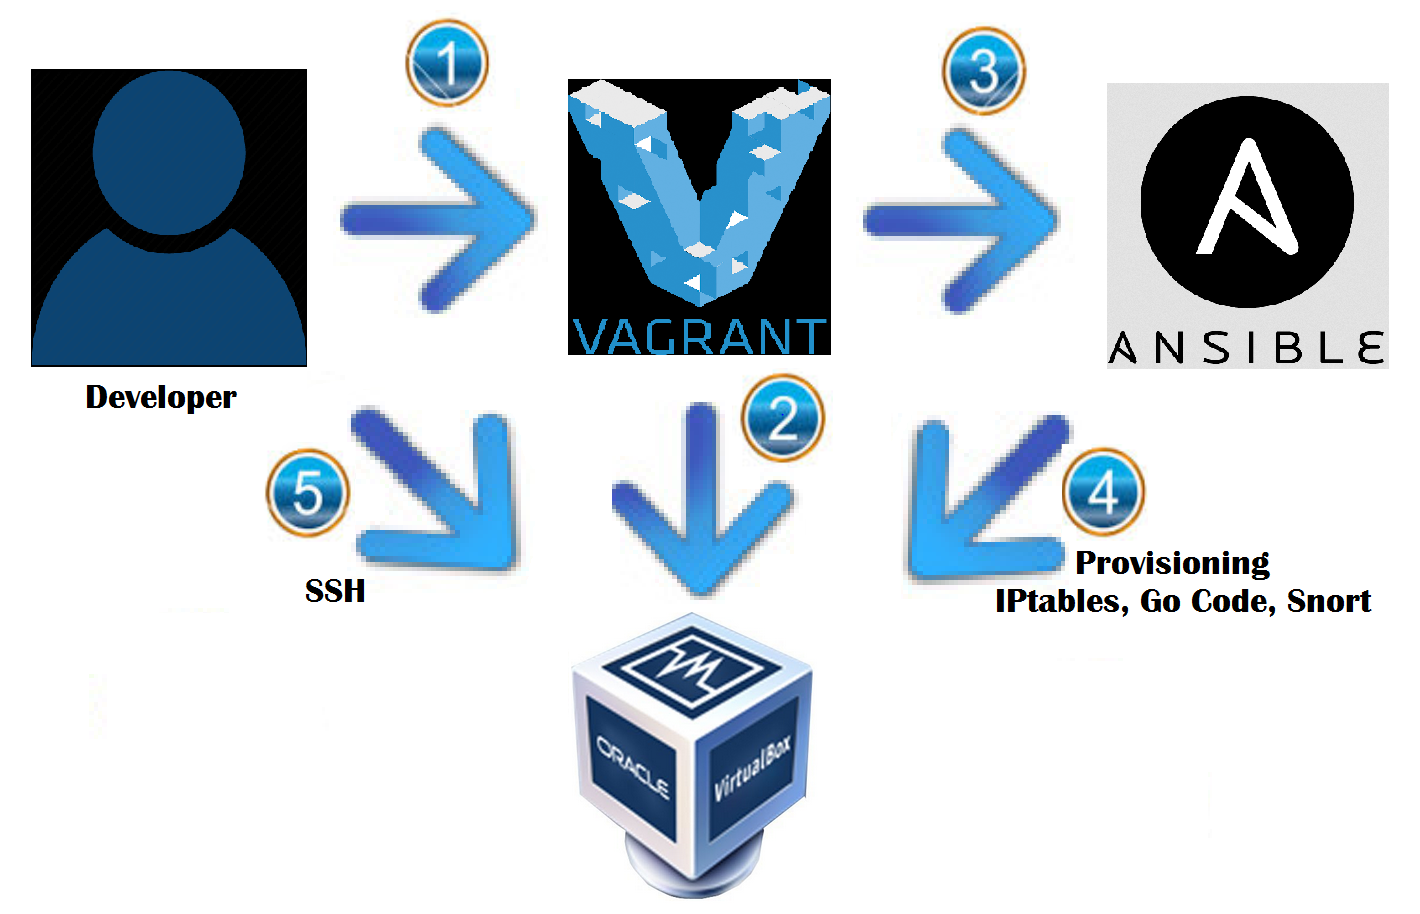
\includegraphics[width=\linewidth]{figures/Vagrant.png}
%\captionof{figure}{\color{Black} Vagrant Environment}
\end{multicols}
